\chapter{Acuity Prediction Models}
\label{ch:acuity_models}

Three conceptually different routes from optical quality to a clinical acuity number
are implemented and compared throughout this project, per an explicit ``investigate
several, do not assume one'' brief. None is asserted as \emph{the} correct model ---
Chapter~\ref{ch:validation} reports which one (if any) tracks published clinical data
best.

\section{Route 1: MTF-cutoff-based MAR}

A resolvable grating at cutoff frequency $f_c$ (cycles/degree) corresponds to a
minimum angle of resolution
\begin{equation}
\text{MAR (arcmin)} = \frac{30}{f_c}
\end{equation}
(exact geometric identity: $1$ cycle $=2$ arcmin of grating period, and $20/20$
acuity is defined as $1$ arcmin MAR $\leftrightarrow 30$\,cpd cutoff). Applied at both
MTF50 and MTF10 as two candidate threshold criteria, since no single universally-agreed
MTF threshold exists for acuity prediction.

\section{Route 2: VSOTF-adjusted acuity}

The Visual Strehl ratio via the OTF (VSOTF; Thibos et al./Iskander, approximate
fidelity here) weights the \emph{real part} of the actual and diffraction-limited OTF
by the neural CSF, then compares CSF-weighted areas rather than raw peak PSF
intensity:
\begin{equation}
\text{VSOTF} = \frac{\int \text{Re}[\text{OTF}_{actual}(f)]\,\text{CSF}(f)\,df}
{\int \text{Re}[\text{OTF}_{DL}(f)]\,\text{CSF}(f)\,df}.
\end{equation}
This asks ``how much of the optically-transmitted contrast survives at the spatial
frequencies human vision actually uses'' rather than reading a single, possibly-lucky
peak (cf.\ the Strehl instability of Chapter~\ref{ch:mtf_strehl}). Applied as a
correction to the MTF10-based MAR:
$\text{MAR}_{VSOTF} = \text{MAR}_{10}/\text{clip}(\text{VSOTF},0.25,2.0)^{0.1}$.

\section{Route 3: photon-noise (Rose--DeVries) SNR bound}

A first-principles scaling argument: in the DeVries--Rose (mesopic/low-light) regime,
detectable contrast threshold scales as $1/\sqrt{\text{flux}}$, so relative
sensitivity scales as $\sqrt{\text{flux}}$, giving a photon-noise-limited MAR bound
relative to a reference condition. This reproduces the \emph{scaling law} exactly
(first-principles Poisson SNR $\sim\sqrt{N}$); it does not reproduce Rose's original
absolute threshold constants.

\section{The cited brightness correction}

An additive logMAR penalty below the Weber-law knee, replacing an earlier uncited
$(\text{SNR})^{0.05}$ exponent term (kept, unmodified, as a legacy comparison point):
\begin{equation}
\Delta\text{logMAR} = \begin{cases} 0 & \text{Td} \ge 300 \\
0.060\,\log_{10}(300/\text{Td}) & \text{Td} < 300 \end{cases}
\label{eq:brightness-logmar}
\end{equation}
The $300$\,Td knee is Van Nes \& Bouman (1967), verified directly against the primary
abstract (Chapter~\ref{ch:brightness_reconciliation}); the $0.060$ slope is Tidbury,
Czanner \& Newsham (2016), verified directly against full text ($p<0.001$, $N=28$),
cross-checked against Sheedy, Bailey \& Raasch (1984)'s independently-derived
$\approx0.0664$ (secondary-sourced only, since the primary text is paywalled).

\begin{figure}[htbp]
\centering
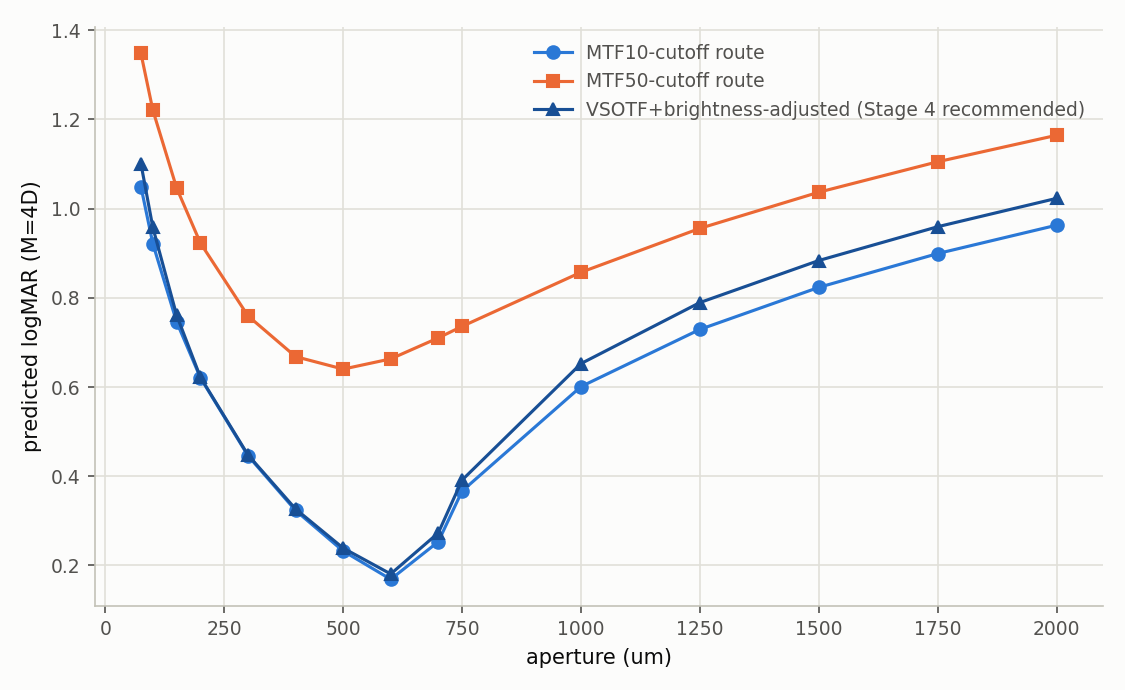
\includegraphics[width=0.85\textwidth]{figures/fig_acuity_models_comparison.png}
\caption{Predicted logMAR vs.\ aperture, all three acuity-model routes, at a representative myopia level.}
\label{fig:acuity-models}
\end{figure}

The brightness correction (Equation~\ref{eq:brightness-logmar}) is visible mainly at
small-to-mid apertures, where retinal illuminance dips below the $300$\,Td knee even
at bright scene luminance; it is negligible at large apertures, where illuminance
stays above the knee at every luminance tested here. At the $M=4\,$D optimum aperture
($400\um$), the recommended predictor moves from $0.414$ logMAR ($10{,}000\,\text{cd/m}^2$
scene, $\text{Td}=1257$) to $0.497$ logMAR ($100\,\text{cd/m}^2$, $\text{Td}=12.6$) ---
a real $\approx0.08$ logMAR brightness effect, versus the legacy term's essentially
flat $0.399\to0.403$.
